\documentclass[]{beamer}
\usepackage[T1]{fontenc}
\usepackage[utf8]{inputenc}
\usepackage{lmodern}
\usepackage[italian]{babel}
\usepackage{mathrsfs}

\title{Le onde luminose}
\author{\texorpdfstring{Mattia Cozzi\newline\href{mailto:cozzimattia@gmail.com}{\texttt{cozzimattia@gmail.com}}}{Mattia Cozzi}}
\date{a.s.~2023/2024}

%\documentclass[handout]{beamer}     %usare questa classe per generare l'handout
%\usepackage{pgfpages}   %per mostrare più quadri nella stessa pagina
%\pgfpagesuselayout{4 on 1}[a4paper,border shrink=5mm,landscape]
\usetheme{Singapore}
%\useoutertheme[left]{sidebar} %elementi intorno alle diapositive
\setbeamercovered{dynamic} %modifica l'aspetto del testo grigetto delle diapositive future. Argomenti: invisible/transparent/dynamic
\usecolortheme{orchid}
%COLORE PRINCIPALE
% \definecolor{marroncino}{RGB}{156, 26, 0} % UBC Blue (primary)
% \setbeamercolor{structure}{fg=marroncino} % itemize, enumerate, etc

\theoremstyle{plain}
\newtheorem{teorema}{Teorema}

\usepackage{tikz}
\usepackage{circuitikz}

\usepackage{pgf,pgfplots,graphicx}
\usetikzlibrary{angles,quotes,arrows,shapes,decorations.markings}
\pgfplotsset{compat=1.15}
\usepgfplotslibrary{units,fillbetween} % to add units easily to axis

\newcommand{\fem}{f_{em}}

\def\angolo[#1](#2)(#3:#4:#5)% Syntax: [draw options] (center) (initial angle:final angle:radius)
    { \draw[#1] ($(#2)+({#5*cos(#3)},{#5*sin(#3)})$) arc (#3:#4:#5); }


\begin{document}

\begin{frame}
  \titlepage
\end{frame}





\begin{frame}
\frametitle{Contenuti}
\tableofcontents
\end{frame}


\section{Teorie}


\begin{frame}
\frametitle{XVII secolo}
\begin{columns}
\begin{column}{0.2\textwidth}
\visible<1->{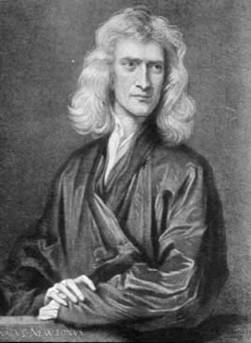
\includegraphics[width=\columnwidth]{img/newton.jpg}}
~
\visible<2->{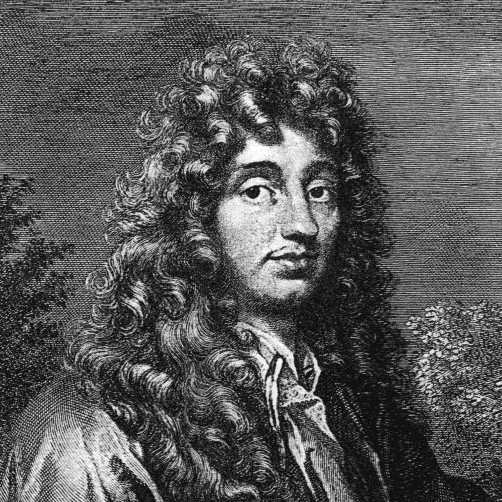
\includegraphics[width=\columnwidth]{img/huygens.jpg}}
\end{column}
\begin{column}{0.7\textwidth}
Nel XVII secolo furono proposte due teorie concorrenti in merito alla natura della luce:
\begin{itemize}
\item<1-> il \alert<1>{modello corpuscolare} di Newton (ispirato da Pierre Gassendi), per cui la luce è un flusso di particelle microscopiche emesse dalle sorgenti luminose;\pause
\item<2-> il \alert<2>{modello ondulatorio} di Huygens (ispirato da Robert Hooke), per cui la luce è un'onda (similmente al suono).
\end{itemize}

\end{column}
\end{columns}
\end{frame}



\begin{frame}
\frametitle{Teorie rivali (1)}
Le due teorie differiscono nel fatto che:
\begin{itemize}
  \item nella teoria corpuscolare abbiamo un \alert<1>{movimento di materia};\pause
  \item nella teoria ondulatoria abbiamo invece un \alert<2>{trasporto di energia} ma non di materia.
\end{itemize}
~\pause\\
La teoria corpuscolare prevedeva inoltre che la luce fosse \alert<1>{più veloce nell'acqua che nel vuoto}, mentre la teoria ondulatoria prevedeva il contrario.\\~\pause\\
Tendenzialmente in fisica una teoria viene ritenuta migliore di un'altra quando riesce a spiegare con chiarezza un numero maggiore di fenomeni.
\end{frame}


\begin{frame}
\frametitle{Teorie rivali (2)}
Il modello corpuscolare (aiutato anche dalla fama di Newton) permetteva di spiegare le ombre, la polarizzazione, la riflessione e la rifrazione.\pause\\~\\
Il modello ondulatorio, che spiegava polarizzazione, riflessione e rifrazione, era considerato poco convincente, poiché non era chiaro di che tipo di onda si trattasse e in quale mezzo si dovesse propagare (venne proposto da Huygens un mezzo \emph{ad hoc}, l'etere luminifero).
\pause\\~\\
Buona parte della comunità scientifica optò pertanto per il modello corpuscolare.
\end{frame}


\begin{frame}
\frametitle{XIX secolo}
\begin{columns}
\begin{column}{0.2\textwidth}
\visible<1->{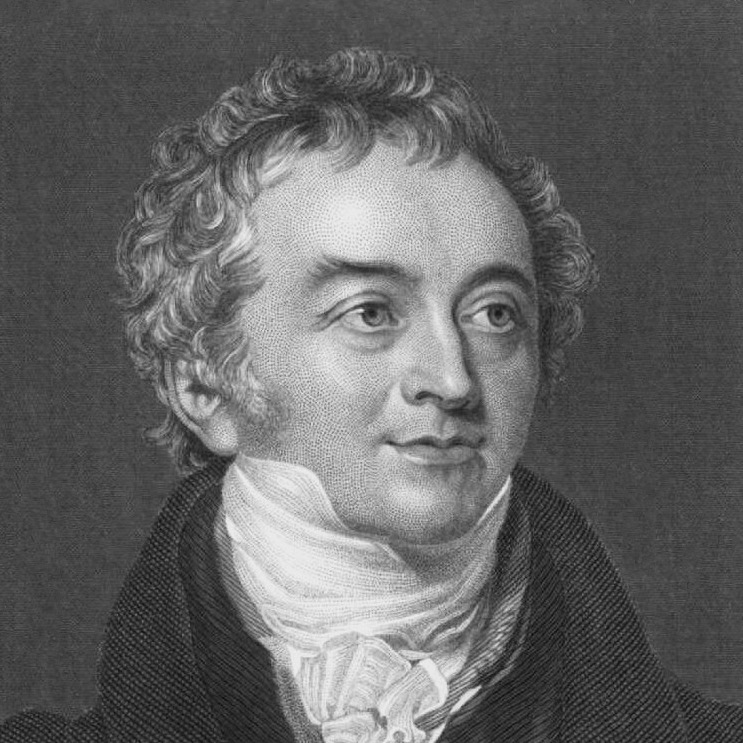
\includegraphics[width=\columnwidth]{img/young.jpg}}
~
\visible<3->{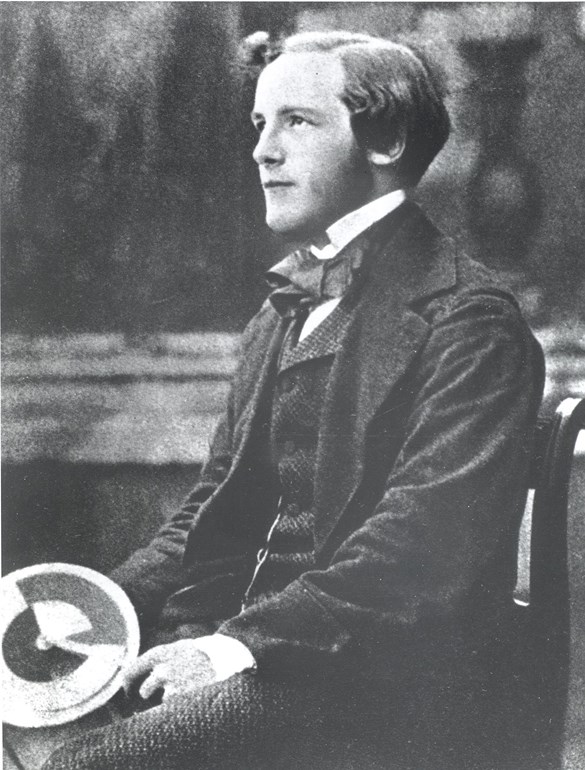
\includegraphics[width=\columnwidth]{img/maxwell.jpg}}
\end{column}
\begin{column}{0.7\textwidth}
La situazione cambia nel XIX secolo, quando:
\begin{itemize}
  \item<1-> Thomas Young (1801) dimostra che la luce presenta il \alert<1>{fenomeno dell'interferenza, tipico unicamente delle onde};
  \item<2-> Léon Foucault e Hippolyte Fizeau (1850) dimostrano che la luce nell'acqua è più lenta che nell'aria, \alert<2>{in accordo con la teoria ondulatoria};
  \item<3-> James Clerk Maxwell (1862 e 1873) dimostra che \alert<3>{la luce è un'onda elettromagnetica} che si propaga anche nel vuoto.
\end{itemize}

\end{column}
\end{columns}
\end{frame}


\begin{frame}
\frametitle{L'esperimento di Young (1801)}
\begin{figure}
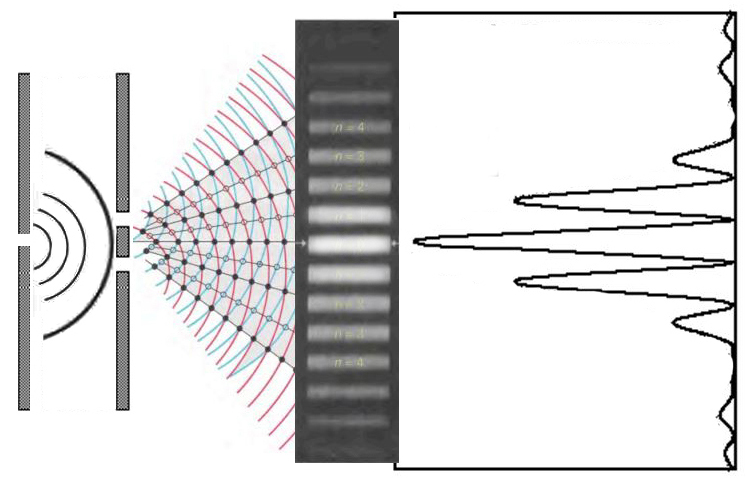
\includegraphics[width=.7\columnwidth]{img/esperimentoyoung.jpg}
\end{figure}

Le due fenditure si comportano da sorgenti coerenti di onde, e si osserva una \alert{figura di interferenza} dovuta all'alternanza tra interferenza costruttiva ed interferenza distruttiva. 

\begin{center}
\href{gif/young.gif}{\beamergotobutton{GIF: L'esperimento di Young}}
\end{center}
\end{frame}



\begin{frame}
\frametitle{XX secolo}
\begin{columns}
\begin{column}{0.2\textwidth}
\visible<1->{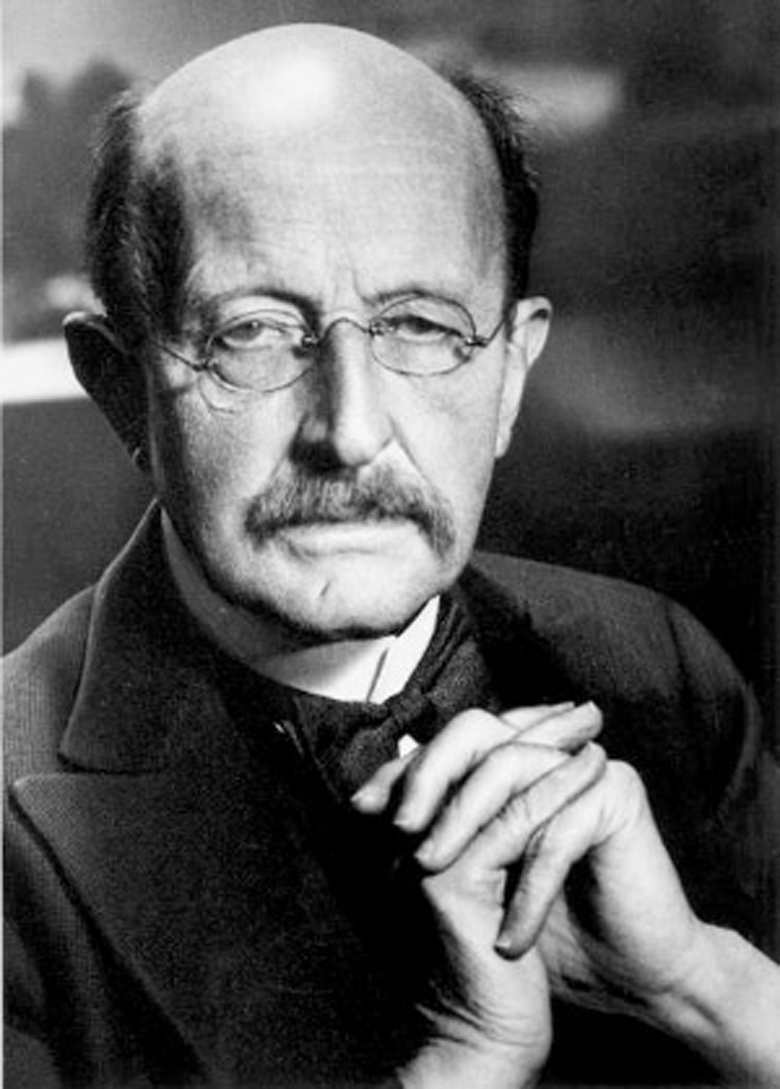
\includegraphics[width=\columnwidth]{img/planck.jpg}}
~
\visible<2->{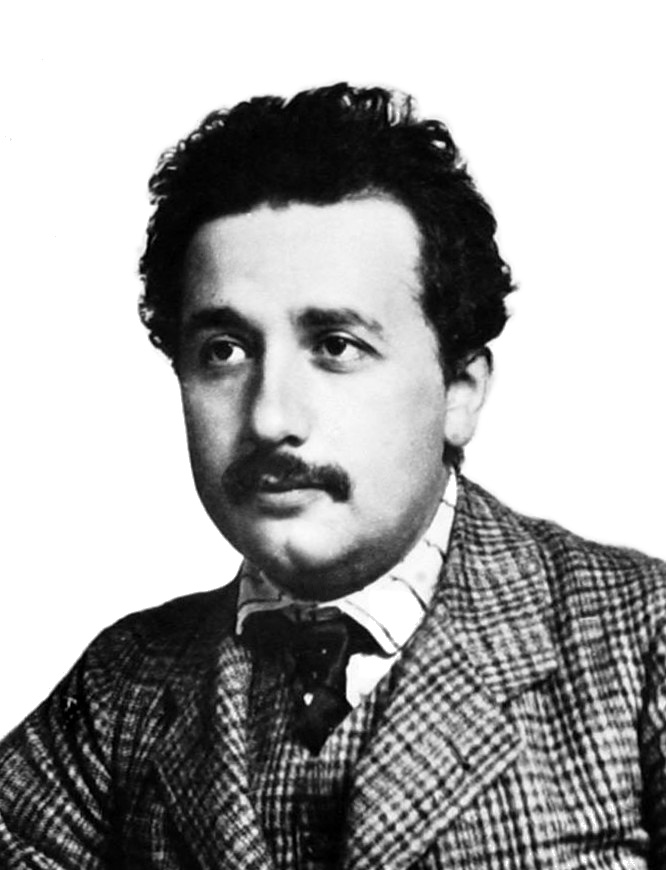
\includegraphics[width=\columnwidth]{img/einstein.jpg}}
\end{column}
\begin{column}{0.7\textwidth}
\begin{itemize}
  \item<1-> Planck (1900) ipotizza che la radiazione elettromagnetica sia formata da quanti di energia;
  \item<2-> Einstein (1905), analizzando l'effetto fotoelettrico, propone che la luce si comporti sia come onda elettromagnetica, sia come flusso di particelle (\emph{fotoni}).
\end{itemize}
\visible<3>{Oggi si ritiene che entrambi i modelli siano validi: \alert{in alcune situazioni la luce si comporta come un'onda, in altre come insieme di corpuscoli}.}
\end{column}
\end{columns}
\end{frame}


\section{Velocità}

\begin{frame}
\frametitle{Velocità della luce nel vuoto}
La velocità della luce nel vuoto è una costante universale indicata con $ c $:

\begin{center}
\colorbox{blue!30}{$ c = 3,00 \times 10^8 \, \frac{m}{s} $} 
\end{center}
\end{frame}

\begin{frame}
\frametitle{Velocità della luce nei mezzi trasparenti}
Nei mezzi trasparenti la velocità $ v $ della luce è sempre minore di $ c $ e permette di definire l'\alert{indice di rifrazione}:
\begin{center}
\colorbox{blue!30}{$ n = \dfrac{c}{v} $} 
\end{center}\pause
Poiché $ v $ è sempre minore di $ c $, l'indice di rifrazione di un mezzo è sempre maggiore di 1.
\begin{center}
$ n_{aria} = 1,0003$~~~~ $ n_{acqua} = 1,33$~~~~$ n_{vetro} = 1,5-1,9$
\end{center}
\end{frame}



\section{Energia}


\begin{frame}
  \frametitle{Energia}
  In quanto onda, la luce trasporta energia:
  \begin{columns}
    \begin{column}{0.3\textwidth}
      \begin{figure}
        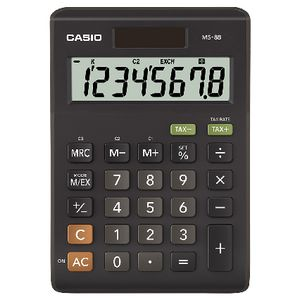
\includegraphics[width=\columnwidth]{img/calcolatrice.jpg}
      \end{figure}
    \end{column}
    \begin{column}{0.3\textwidth}
      \visible<2-3>{\begin{figure}
        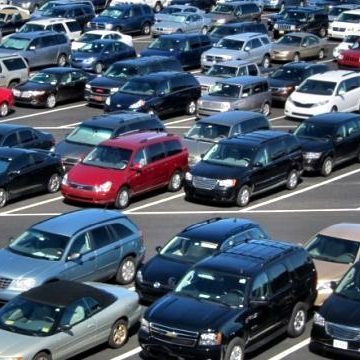
\includegraphics[width=\columnwidth]{img/parcheggio.jpg}
      \end{figure}
      }
    \end{column}
    \begin{column}{0.3\textwidth}
      \visible<3>{\begin{figure}
        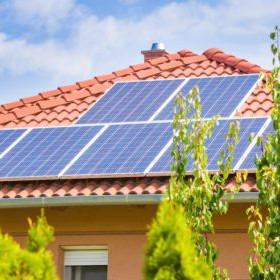
\includegraphics[width=\columnwidth]{img/pannelli.jpg}
      \end{figure}
      }
    \end{column}
  \end{columns}
\end{frame}


\begin{frame}
\frametitle{Irradiamento}

\begin{block}{Irradiamento}
Se una superficie $ A $ in un certo intervallo di tempo $ \Delta t $ è attraversata perpendicolarmente da un'onda luminosa che trasporta un'energia $ E $, allora:
\begin{center}
\colorbox{blue!30}{$ E_e = \dfrac{E}{A\Delta t} $}
\end{center}
Come l'intensità sonora (di cui è l'analogo), l'irradiamento si misura in $ \dfrac{W}{m^2} $.
\end{block}
\end{frame}



\begin{frame}
\frametitle{Esercizio}
\begin{exampleblock}{Irradiamento massimo}
{\small Gli standard di sicurezza prevedono che per tutelare gli occhi dei lavoratori esposti ai raggi UV sia imposto un limite di $ 10 \, kJ/m^2 $ per una giornata di 8 ore di lavoro.

Stima l'ordine di grandezza dell'irradiamento massimo a cui possono essere sottoposti per unità di superficie.}
\end{exampleblock}
\end{frame}


\section{Riflessione}

\begin{frame}
\frametitle{Leggi della riflessione}
Queste leggi sono state formulate per la prima volta da René Descartes (Cartesio).\pause
\begin{enumerate}
  \item Il raggio incidente, il raggio riflesso e la perpendicolare (normale) alla superficie riflettente giacciono sullo stesso piano.\pause
  \item L'angolo di incidenza $ \hat{i} $ è uguale all'angolo di riflessione $ \hat{r} $.
\end{enumerate}
\begin{figure}
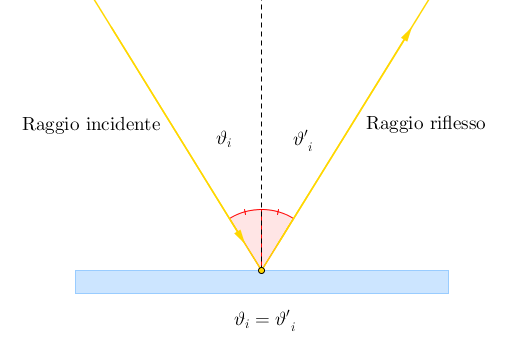
\includegraphics[width=.7\columnwidth]{img/riflessione.png}
\end{figure}
\end{frame}


\begin{frame}
\frametitle{Riflessione su uno specchio piano}
\begin{columns}
\begin{column}{0.5\textwidth}
\begin{figure}
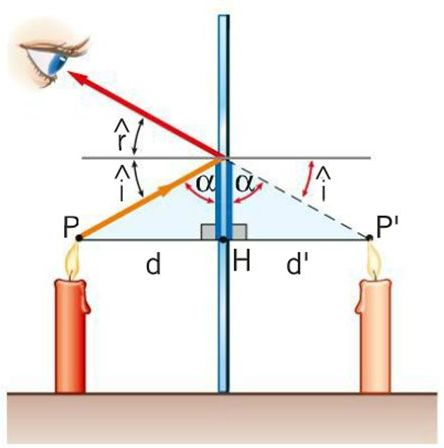
\includegraphics[width=\columnwidth]{img/specchio.jpg}
\end{figure}
\end{column}
\begin{column}{0.5\textwidth}
L'immagine che \emph<1>{sembra} provenire da dietro lo specchio è detta \alert<1>{immagine virtuale}.\pause

~

È dove convergono i \alert<2>{prolungamenti dei raggi} dopo essere stati riflessi.\pause

~

Come si comporta invece uno specchio non piano?
\end{column}
\end{columns}
\end{frame}


\begin{frame}
\frametitle{Specchi parabolici}
Gli specchi parabolici hanno la caratteristica di convogliare tutti i raggi paralleli al loro asse verso un punto, il \alert{fuoco}.
\begin{figure}
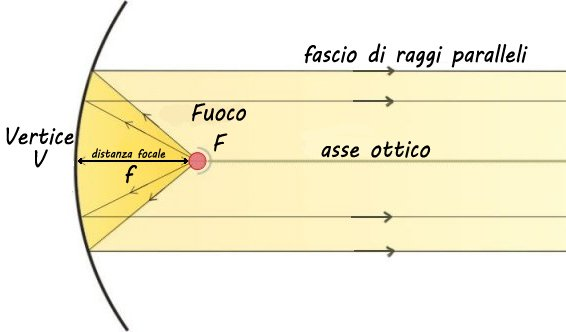
\includegraphics[width=.8\columnwidth]{img/specchioparabolico.jpg}
\end{figure}
\end{frame}


\begin{frame}
\frametitle{Specchi sferici}
Specchi sferici con piccola apertura approssimano bene gli specchi parabolici e le loro caratteristiche.
\begin{figure}
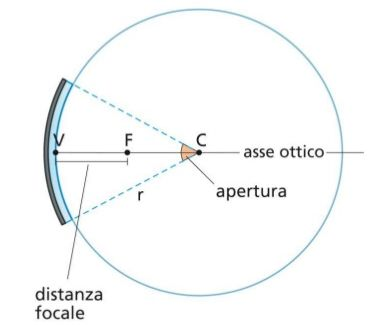
\includegraphics[width=.5\columnwidth]{img/specchiosferico.jpg}
\end{figure}
\end{frame}


\begin{frame}
\frametitle{Il fuoco negli specchi sferici}
\begin{columns}
\begin{column}{0.45\textwidth}
\begin{figure}
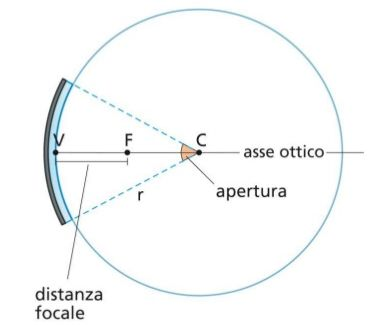
\includegraphics[width=\columnwidth]{img/specchiosferico.jpg}
\end{figure}
\end{column}
\begin{column}{0.5\textwidth}
Negli specchi sferici \alert<1>{la distanza focale è la metà del raggio} dello specchio.
\begin{center}
\colorbox{blue!30}{$ f = \dfrac{r}{2} $}
\end{center}
\end{column}
\end{columns}
\end{frame}

\section{Rifrazione}


\begin{frame}
\frametitle{Rifrazione}
\begin{columns}
\begin{column}{0.3\textwidth}
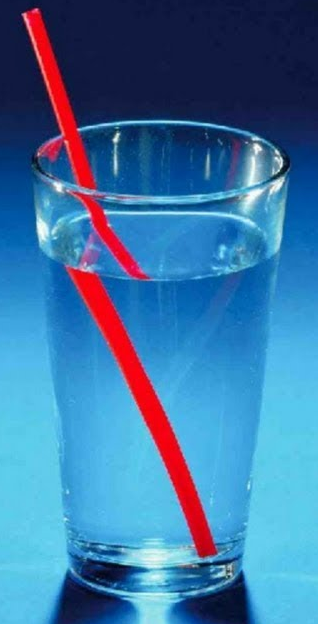
\includegraphics[width=\columnwidth]{img/rifrazione.png}
\end{column}
\begin{column}{0.6\textwidth}
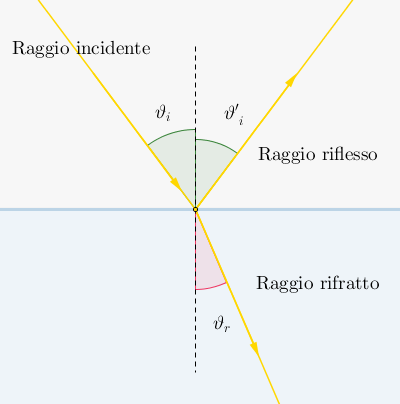
\includegraphics[width=\columnwidth]{img/snell.png}
\end{column}
\end{columns}
\end{frame}


\begin{frame}
\frametitle{Leggi della rifrazione}
Quando un raggio di luce attraversa la superficie di separazione tra due mezzi trasparenti con indici di rifrazione $ n_1 $ e $ n_2 $, esso viene rifratto.
\begin{enumerate}
  \item Il raggio incidente, il raggio rifratto e la perpendicolare (normale) alla superficie riflettente giacciono sullo stesso piano.
  \item Legge di Snell:
  \begin{center}
\colorbox{blue!30}{$ n_1 \cdot \sin \hat{i} = n_2 \cdot\sin \hat{r} $} 
\end{center}
\end{enumerate}
\end{frame}


\begin{frame}
\frametitle{Indici di rifrazione e angoli limite}
\begin{table}[htp]\centering
  \begin{tabular}{ccc}\hline\rule{0pt}{3ex}
        \textbf{Materiale}    & \textbf{n}  & \textbf{Angolo limite}\\\hline\rule{0pt}{3ex}
        ghiaccio      & 1,31      & $ 49,8^\circ $\\\hline\rule{0pt}{3ex}
        acqua         & 1,33      & $ 48,6^\circ $\\\hline\rule{0pt}{3ex}
        alcol etilico & 1,36      & $ 47,2^\circ $ \\\hline\rule{0pt}{3ex}
        plexiglas     & 1,49      & $ 42,2^\circ $\\\hline\rule{0pt}{3ex}
        vetro         & 1,50-1,90 & $ 31,9^\circ-41,5^\circ $\\\hline\rule{0pt}{3ex}
        diamante      & 2,42      & $ 24,4^\circ $\\\hline
  \end{tabular}
\end{table}
\end{frame}


\begin{frame}
\frametitle{Esercizi}
\begin{exampleblock}{Angolo di rifrazione}
{\small Un raggio di luce incide sulla superficie di separazione aria-diamante (in quest'ordine) formando un angolo di $ 45^\circ $ con la normale alla superficie.

Calcola l'angolo di rifrazione.\hspace*{\fill}[$ 17^\circ $]}
\end{exampleblock}

~

\begin{exampleblock}{Separazione della luce nei colori}
{\small Su una lastra di cristallo spessa $ 0,10 \, m $ incide un fascio di luce solare con un angolo di $ 60^\circ $. L'indice di rifrazione del materiale è di 1,607 per la luce violetta, mentre è di 1,569 per la luce rossa.

\begin{itemize}
  \item Quanto valgono gli angoli di rifrazione per i due raggi?\hspace*{\fill}[$ 33^\circ, 34^\circ $]
  \item Rappresenta la situazione con un disegno.
  \item Di quanto sono distanziati i punti di uscita dei fasci di questi due colori quando riemergono dal vetro?\hspace*{\fill}[$ 2,2 \times 10^{-3} \, m $]
\end{itemize}
}
\end{exampleblock}
\end{frame}



\begin{frame}
\frametitle{L'angolo limite}
Dalla legge di Snell si deduce che se $ n_1 > n_2 $, allora $ \hat{r} > \hat{i} $ e i raggi si allontanano dalla retta perpendicolare.

~

Possiamo portare questa situazione all'estremo, fino a rendere $ \hat{r} $ un angolo retto.
\begin{figure}
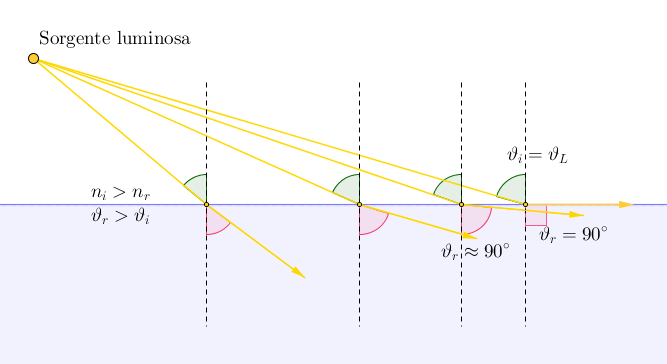
\includegraphics[width=.8\columnwidth]{img/angololimite.png}
\end{figure}
\end{frame}

\begin{frame}
\frametitle{Leggi della riflessione totale}
Diciamo \alert{angolo limite} l'angolo di incidenza $ \hat{i}_L $ per cui $ \hat{r} = 90^\circ $.\pause

~

Partiamo dalla legge di Snell, ricordando che $ \sin 90^\circ = 1 $:
\[  n_1 \cdot \sin \hat{i}_L = n_2 \cdot\sin 90^\circ \]\pause
\[ \sin\hat{i}_L = \frac{n_2}{n_1} \]\pause
\begin{center}
\colorbox{blue!30}{$\displaystyle \hat{i}_L = \arcsin\left(\frac{n_2}{n_1}\right) $}
\end{center}
\begin{center}
  \href{https://www.youtube.com/watch?v=NAaHPRsveJk}{\beamergotobutton{Video: esperimento}}
\end{center}


\end{frame}


\begin{frame}
\frametitle{Riflessione totale}
Se l'angolo di incidenza è superiore all'angolo limite, la rifrazione non può avvenire e si assiste al fenomeno della \alert{riflessione totale}.

\begin{figure}
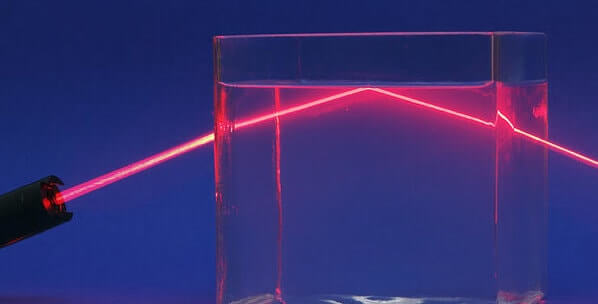
\includegraphics[width=.8\columnwidth]{img/riflessionetotale.jpg}
\end{figure}
\end{frame}




\begin{frame}
\frametitle{Esercizio}
\begin{exampleblock}{Angolo di rifrazione}
{\small Un raggio di luce attraversa le pareti in vetro ($ n_1 = 1,60  $) di una vasca di acqua salata ($ n_2 = 1,55 $)

Quanto vale l'angolo limite per un raggio di luce che passa dal vetro all'acqua salata?\hspace*{\fill}[$ 76^\circ $]}
\end{exampleblock}
\end{frame}


% \section{Young}





\section{Spettro}

\begin{frame}
\frametitle{Lunghezze d'onda e colori}
La luce ci appare di diversi colori a seconda della sua \emph{lunghezza d'onda}:
\begin{center}
$ \lambda = \dfrac{c}{f} $
\end{center}\pause
I nostri occhi possono percepire lunghezze d'onda tra i $ 380 $ e i $ 750 \, nm $.
\visible<2>{\begin{figure}
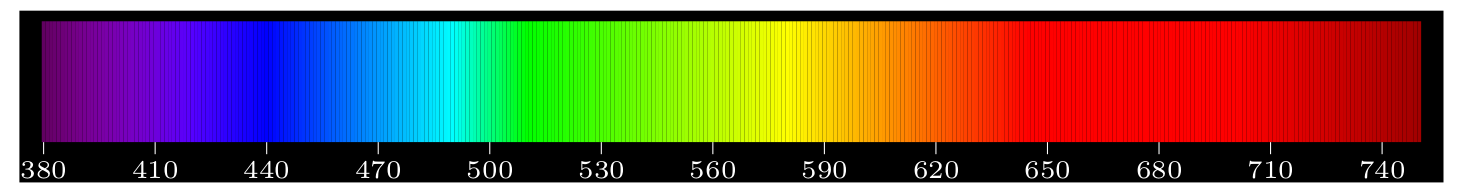
\includegraphics[width=\columnwidth]{img/spettrolum.png}
\end{figure}}
\end{frame}


\begin{frame}
\frametitle{Lo spettro elettromagnetico}
Lo spettro visibile è solo una minuscola parte dello spettro elettromagnetico!
  \begin{figure}
  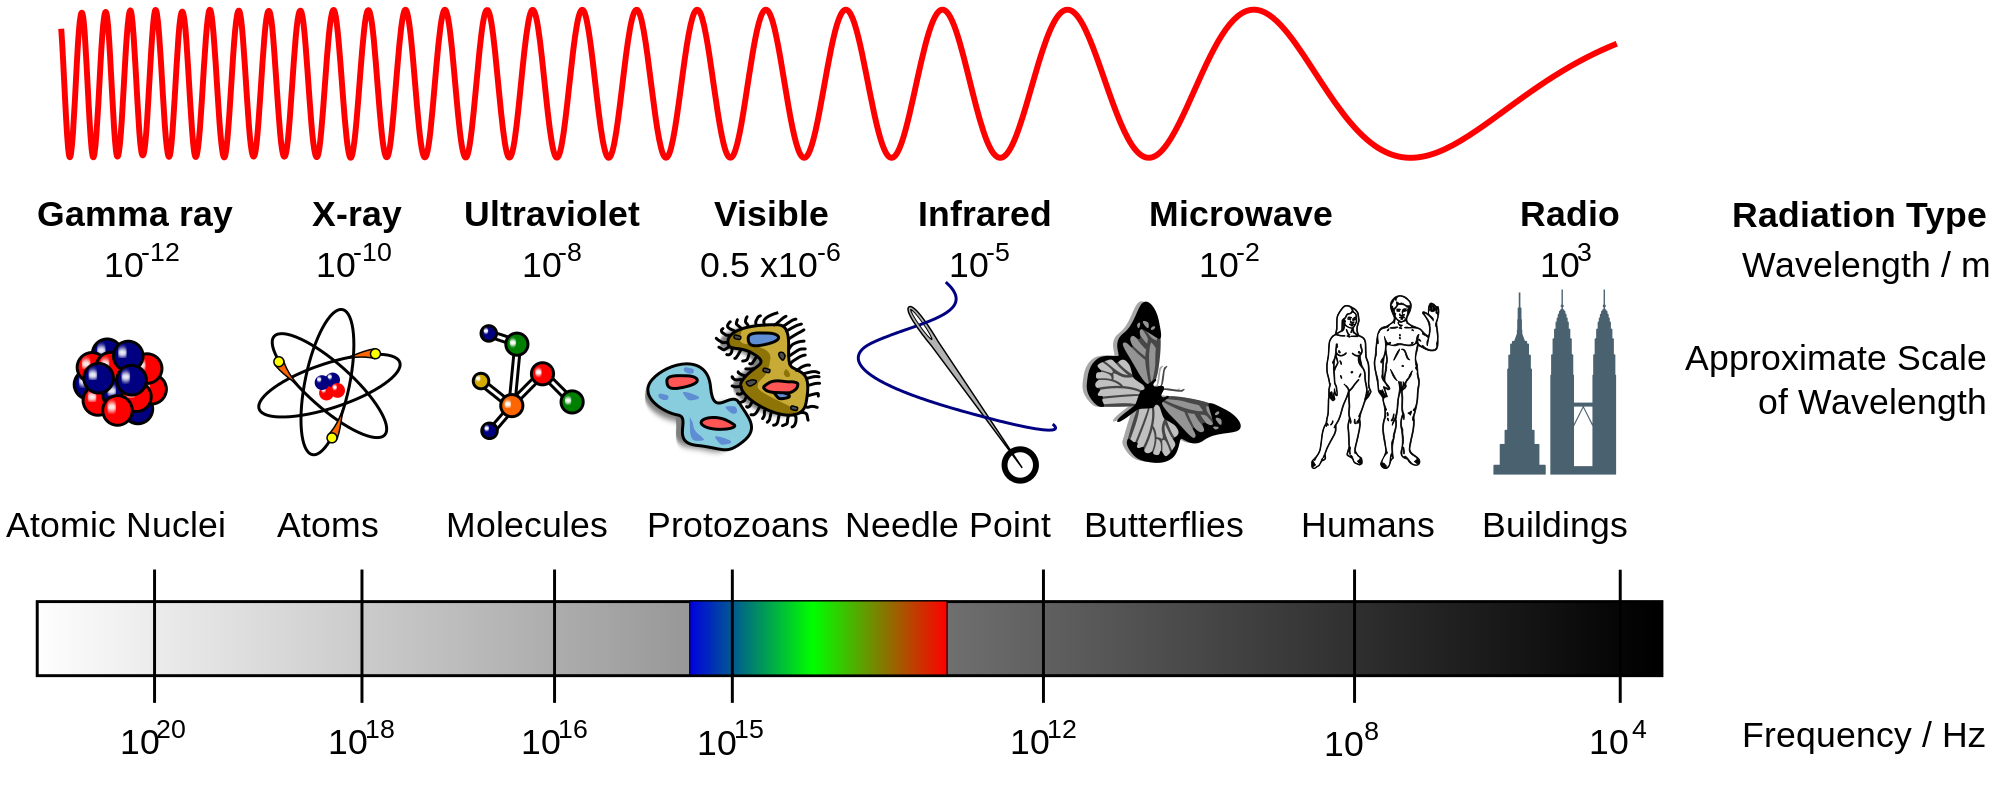
\includegraphics[width=\columnwidth]{img/spettroem.png}
  \end{figure}
\end{frame}






\begin{frame}
\frametitle{Confronto tra luce e suono}


\centering
  \begin{tabular}{l|c|c}
    & \textbf{Luce} & \textbf{Suono} \\\hline\rule{0pt}{3ex}
    Grandezza oscillante & $ \vec{E} $ e $ \vec{B} $ & $ d $ \\\rule{0pt}{3ex}
    Sorgente & Cariche oscillanti & Vibrazioni \\\rule{0pt}{3ex}
    Mezzo & Vuoto e materia & Materia \\\rule{0pt}{3ex}
    Velocità & $ 3 \times 10^8 \,\frac{m}{s} $ & $ 3,4 \times 10^2 \, \frac{m}{s} $ (aria)\\\rule{0pt}{3ex}
    $ f $ percepibile & $ 10^{14} - 10^{15}\, Hz $ & $ 20 - 20000 \, Hz $ \\\rule{0pt}{3ex}
    $ \lambda $ percepibile & $ 380-750 \, nm $ & $ 0,017 - 17 \, m $ (aria)\\
  \end{tabular}
\end{frame}

\section{Ottica geometrica}

\begin{frame}
\frametitle{Raggi di luce}
Anche se sappiamo che la luce è un'onda, in molte situazioni possiamo schematizzarla come segmenti detti \alert<1>{raggi di luce}.\pause

~

Ciò è possibile perché la lunghezza d'onda della luce è molto minore delle dimensioni degli oggetti con cui interagisce. La lunghezza d'onda massima della luce visibile è infatti circa $ 750 \, nm $, cioè meno di 1 milionesimo di metro.\pause

~

Il primo ad occuparsi di ottica in termini scientifici (cioè geometrici) fu Euclide (III secolo a.C.).
\end{frame}



\begin{frame}
\frametitle{Visione}
Come già Euclide aveva capito, \alert<1>{noi vediamo gli oggetti quando la luce che proviene da essi colpisce i nostri occhi}.\pause

~

Questo può accadere perché il corpo emette luce (sorgente luminosa) oppure perché riflette la luce proveniente da una sorgente (corpo illuminato).\pause

~

Il nostro sistema nervoso elabora poi gli stimoli luminosi ricevuti, formando un'\alert<3>{immagine mentale} dell'oggetto.

~

\visible<2->{\begin{figure}
  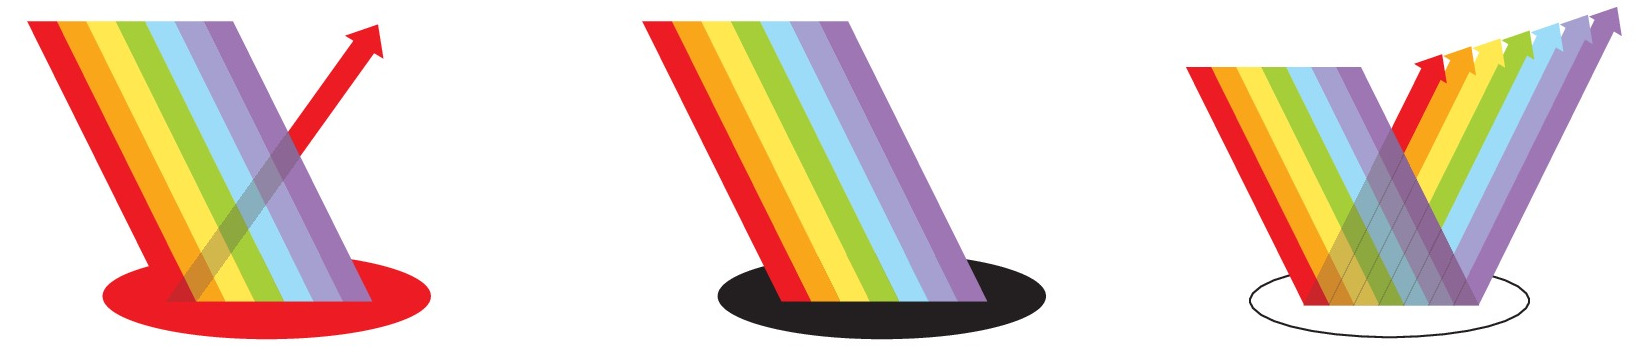
\includegraphics[width=.8\columnwidth]{img/colori.jpg}
\end{figure}}
\end{frame}



\begin{frame}
\frametitle{Specchi piani}
Quando ci vediamo nel riflesso dello specchio, sembra che ci sia una ``copia'' di noi all'interno dello specchio, alla stessa distanza a cui ci troviamo noi.\pause

~

Ogni punto di un oggetto davanti ad uno specchio costituisce una sorgente puntiforme di luce: per vederlo, serve che un raggio che parte dall'oggetto si rifletta sullo specchio e arrivi fino al nostro occhio.

\visible<2->{\begin{figure}
  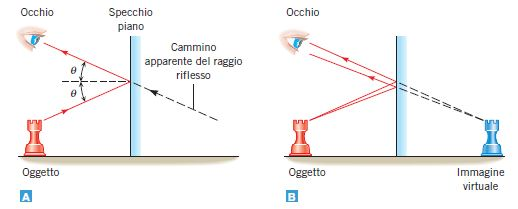
\includegraphics[width=.7\columnwidth]{img/specchiopiano.jpg}
\end{figure}}
\end{frame}


\begin{frame}
\frametitle{Specchi sferici (1)}
\begin{columns}
\begin{column}{0.3\textwidth}
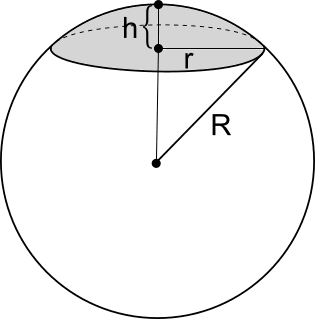
\includegraphics[width=\columnwidth]{img/calotta-sferica.png}
\end{column}
\begin{column}{0.6\textwidth}
  Uno specchio sferico è una calotta, cioè una porzione di superficie di una sfera cava.\pause

  ~

  Se la luce viene riflessa dalla superficie interna della sfera, lo specchio è \alert<2>{concavo}, se la luce è riflessa dalla superficie esterna è \alert<2>{convesso}.
\end{column}
\end{columns}
\end{frame}



\begin{frame}
\frametitle{Specchi sferici (2)}
\begin{columns}
\begin{column}{0.5\textwidth}
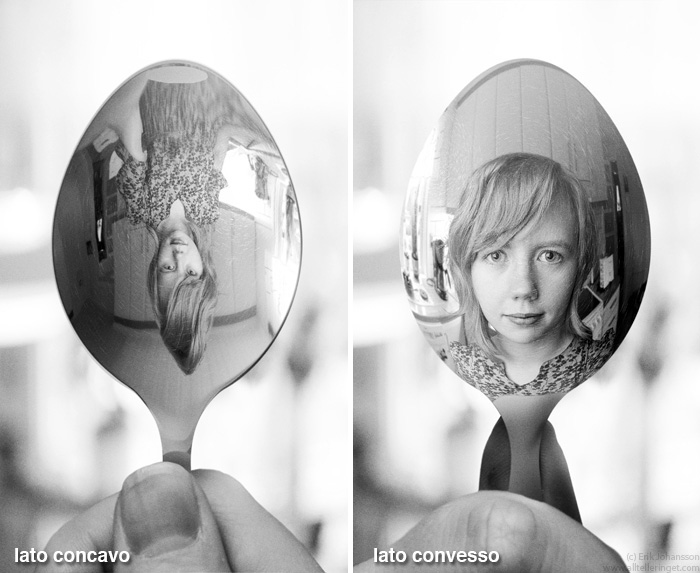
\includegraphics[width=\columnwidth]{img/cucchiaio.jpg}
\end{column}
\begin{column}{0.4\textwidth}
  Se la luce viene riflessa dalla superficie interna della sfera, lo specchio è \alert<2>{concavo}, se la luce è riflessa dalla superficie esterna è \alert<2>{convesso}.
\end{column}
\end{columns}\pause

~

~

Se immaginiamo una sorgente luminosa molto lontana, possiamo affermare che i raggi luminosi che giungono da essa siano tutti paralleli.
\end{frame}



\begin{frame}
\frametitle{Specchi sferici (3)}
Negli specchi sferici, che approssimano quelli parabolici, tutti i raggi incidenti (o i loro prolungamenti) si incontrano nel \alert<1>{fuoco}.

~

\begin{figure}
  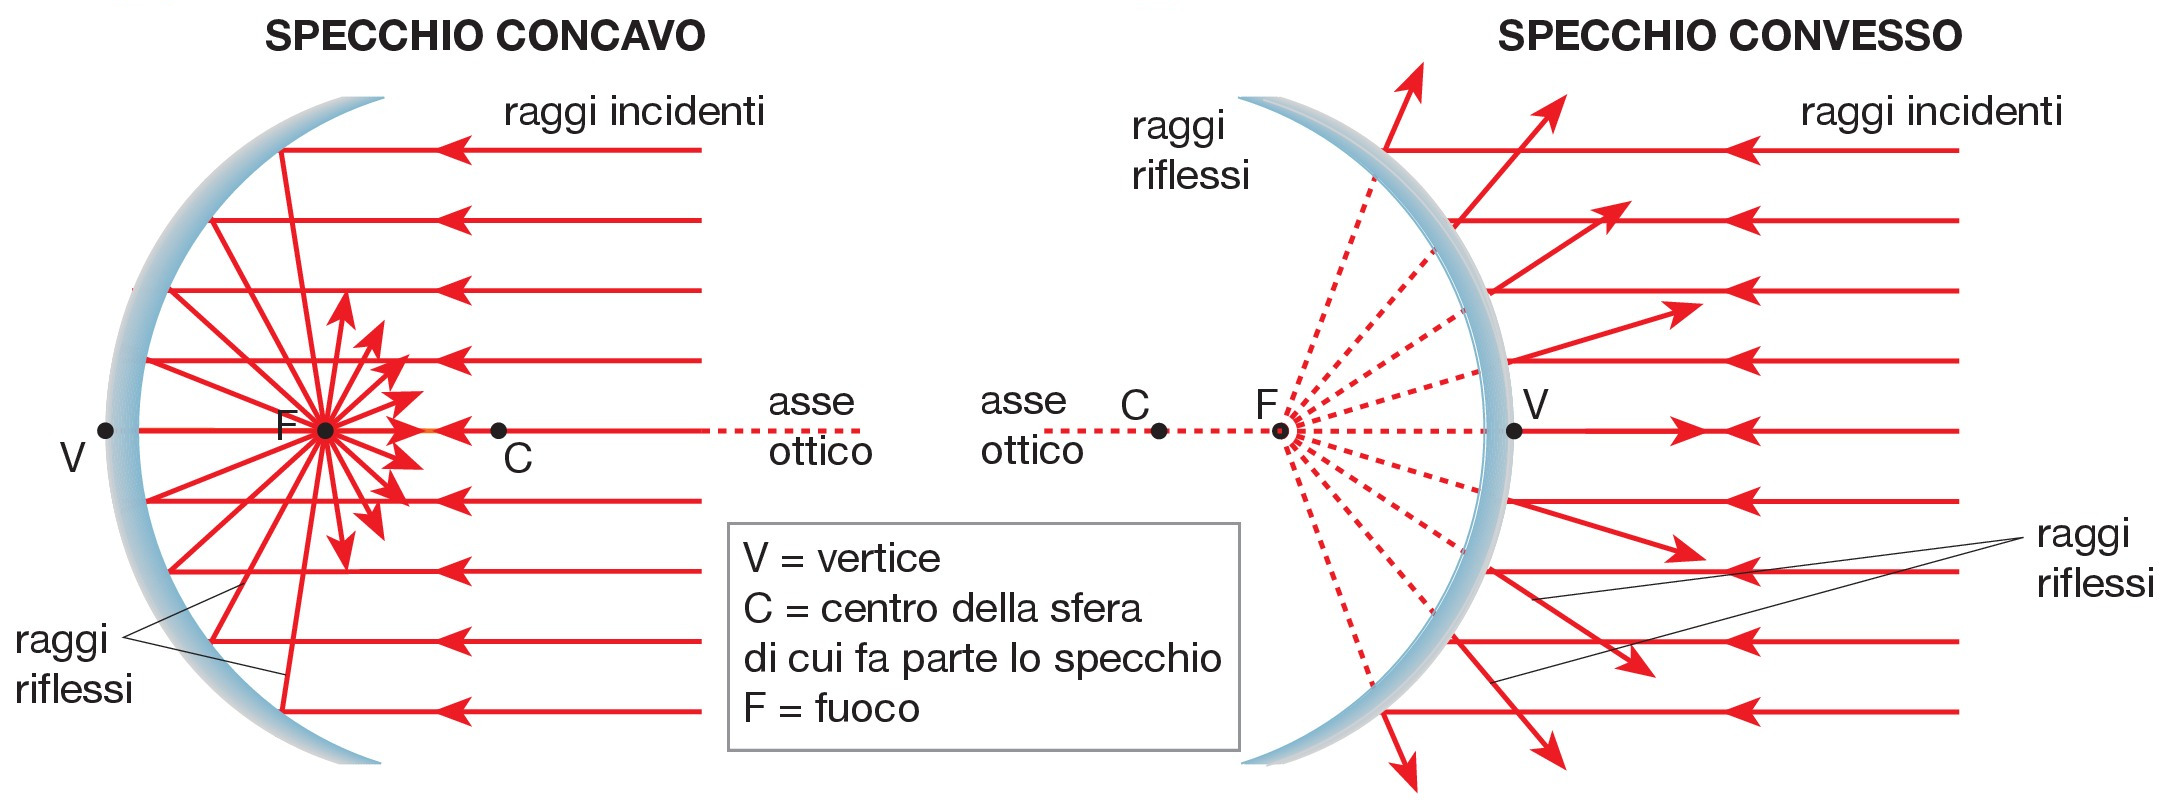
\includegraphics[width=\columnwidth]{img/specchiconcaviconvessi.jpg}
\end{figure}
\end{frame}



\begin{frame}
\frametitle{Il fuoco negli specchi sferici}
\begin{columns}
\begin{column}{0.45\textwidth}
\begin{figure}
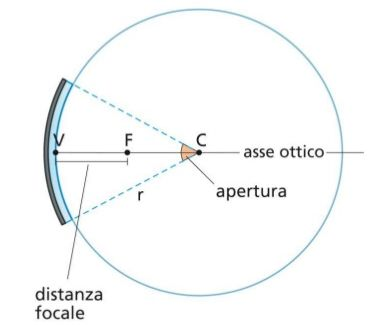
\includegraphics[width=\columnwidth]{img/specchiosferico.jpg}
\end{figure}
\end{column}
\begin{column}{0.5\textwidth}
Negli specchi sferici \alert<1>{la distanza focale è la metà del raggio} dello specchio.
\begin{center}
\colorbox{blue!30}{$ f = \dfrac{r}{2} $}
\end{center}
\end{column}
\end{columns}
\end{frame}

\end{document}
